\documentclass[a4paper, 10pt]{article}%тип документа

%отступы
\usepackage[left=2cm,right=2cm,top=2cm,bottom=3cm,bindingoffset=0cm]{geometry}

%Русский язык
\usepackage[T2A]{fontenc} %кодировка
\usepackage[utf8]{inputenc} %кодировка исходного кода
\usepackage[english,russian]{babel} %локализация и переносы

%Вставка картинок
\usepackage{graphicx}
\graphicspath{{pictures/}}
\DeclareGraphicsExtensions{.pdf,.png,.jpg}

%Графики
\usepackage{pgfplots}
\pgfplotsset{compat=1.9}

%Математика
\usepackage{amsmath, amsfonts, amssymb, amsthm, mathtools}

%Заголовок
\author{
    \vspace*{10cm} \\
    Трунов Владимир \\
    Б01-103}
\title{
\vspace{7cm}
Работа 1.3.1 \\
Определение модуля Юнга на основе исследования деформаций растяжения и изгиба}
\begin{document}
\maketitle
\newpage
\textbf{Цель работы:} экспериментально получить зависимость между напряжением и деформацией (закон Гука) для двух простейших напряженных состояний упругих тел: одноосного растяжения и чистого изгиба; по результатам измерений вычислить модуль Юнга. \\
\textbf{В работе используется:} прибор лермантова, проволока из исследуемого материала, зрительная трубка со шкалой, набор грузов, микрометр, рулетка; во второй части - стойка для изгибания балки, индикатор для измерения величины прогиба, набор исследуемых стержней, грузы, линейка, штангенциркуль.
\center{\textbf{Определение модуля Юнга по измерениям растяжения проволоки (рис.1)}}
\begin{figure}[h]
\center{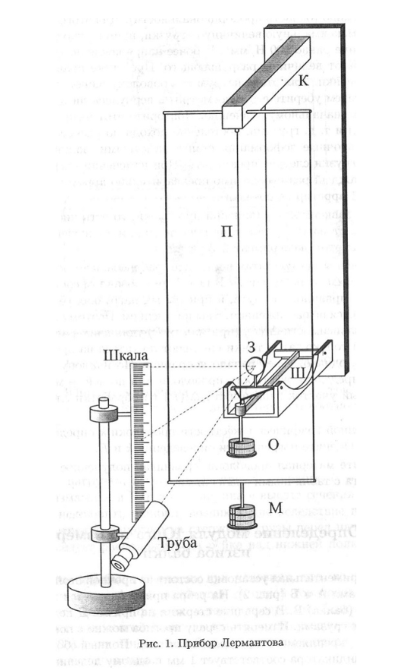
\includegraphics{IMG_1.png}}
\end{figure}
\begin{enumerate}
\item $d = (0,73 \pm 0,01) \text{мм}$. \\
Так как данные о диаметре проволоки были написаны на установке, будем считать их погрешность равной погрешности микрометра (т.е. $\sigma_d = 0,01 \text{мм}$)
\item Измеряем площадь поперечного сечения проволоки
\[S =\dfrac{ \pi (\overline{d})^2}{4} = 0,41 \text{ мм}^2\]
\[\sigma_S = S\sqrt{2\left( \dfrac{\sigma_d}{d}\right) ^2} = 0,008 \text{ мм}^2\]
\[S = (0,41\pm0,008) \text{ мм}^2\]
\item Измеряем длинну проволоки $l = 176  \text{ см}$
\item Направляем зрительную трубу на зеркальце так, чтобы мы четко видели шкалу, тогда свет от шкалы будет падать примерно перпендикулярно шкале на зеркало, поэтому
\[\Delta l =\dfrac{nr}{2h}\]
\[ \sigma_{\Delta l} = \Delta l\sqrt{\left( \dfrac{\sigma_{n}}{n}\right)^2 + \left(\dfrac{\sigma_d}{d}\right)^2+\left(\dfrac{\sigma_h}{h}\right)^2} \]
где $r = 15$ см - длина рычага, разница показаний шкалы - $n$, расстояние от шкалы до проволоки - $h = (138\pm0,1)\text{ см}$.
\item Исходя из того, что $\sigma_{\text{предел}} = 900 \text{ Н}/\text{мм}^2$ получаем, что предельный вес, который можно повесить, чтобы не выйти за пределы $P_{\text{предел}} = 0,3 \sigma_{\text{предел}} S \approx 110,7 H$. 
\item Снимем зависимость удлинения проволоки от массы грузов при увеличении и уменьшении нагрузки 2-3 раза (табл.1). 
\begin{table}
\center{
\begin{tabular}{|c|c|c|c|c|c||c|c|c|c|c|}
\hline
P, Н & 7,92 &10,38 &12,84&15,29 &17,75 &20,21 &22,66 &25,17 &27,568\\
\hline
$\Delta l$, см&1,3 &1,3 &1,1 &1,2 &1,2 &1,2 &1,1 &1,2 &1,2\\ 
\hline
$\sigma_{\Delta l}$&0,028 &0,028 &0,024 &0,026 &0,024 &0,026 &0,026 &0,024 &0,026\\
\hline
\hline
P, Н & 7,92 &10,38 &12,84&15,29 &17,75 &20,21 &22,66 &25,17 &27,568\\
\hline
$\Delta l$, см&1,2 &1,3 &1,1 &1,2 &1,2 &1,2 &1,2 &1,2 &0\\
\hline
$\sigma_{\Delta l}$&0,026 &0,028 &0,024 &0,026 &0,026 &0,026 &0,026 &0,026 &0\\
\hline
\hline
P, Н & 7,92 &10,38 &12,84&15,29 &17,75 &20,21 &22,66 &25,17 &27,568\\
\hline
$\Delta l$&1,4 &1,3 &1,2 &1,2 &1,2 &1,2 &1,2 &1,2 &1,2\\
\hline
$\sigma_{\Delta l}$&0,03 &0,028 &0,026 &0,026 &0,026 &0,026 &0,026 &0,026 &0,026\\
\hline
\hline
P, Н & 7,92 &10,38 &12,84&15,29 &17,75 &20,21 &22,66 &25,17 &27,568\\
\hline
$\Delta l$, см&1,3 &1,2 &1,3 &1,1 &1,5 &1,1 &1 &1,2&0\\
\hline
$\sigma_{\Delta l}$&0,028 &0,026 &0,028 &0,024 &0,03 &0,026 &0,026 &0,026&0\\
\hline
\end{tabular}
}
\caption{Зависимость удлинения проволоки от нагрузки}

\center{
\begin{tabular}{|c|c|c|c|}
\hline
&Значение&$\sigma$&$\varepsilon$\\
\hline
k&$1,73*10^3$ H/м&$0,027*10^3$ Н/м&0,016\\
\hline
E&$18,3*10^{10}$ Па&$ 0,7*10^{10}$ Па&0,04\\
\hline
\end{tabular}
}
\caption{Значения k и E}

\end{table}
\item Построим график зависимости удлинения проволоки от нагрузки. В недеформированном состоянии проволока, как правило, изогнута, и при малых нагрузках её "удлинение" определяется не растяжением, а выпрямлением. Найдем уравнение получившийся прямой по МНК. По наклону прямой определим жесткость проволоки, а по ней - модуль Юнга (табл.2). Начальный участок графика при обработке следует исключить. 
\item По найденной графически жёсткости проволоки найдем модуль Юнга по формуле
\[E = \dfrac{k \cdot l_0}{S}\]
\[\sigma_E = \sqrt{\left( \dfrac{\sigma_{k}}{k} \right)^2 + \left( \dfrac{\sigma_{S}}{S} \right)^2 + \left( \dfrac{\sigma_{l_0}}{l_0} \right)^2 }\]
\end{enumerate}

\begin{center}

    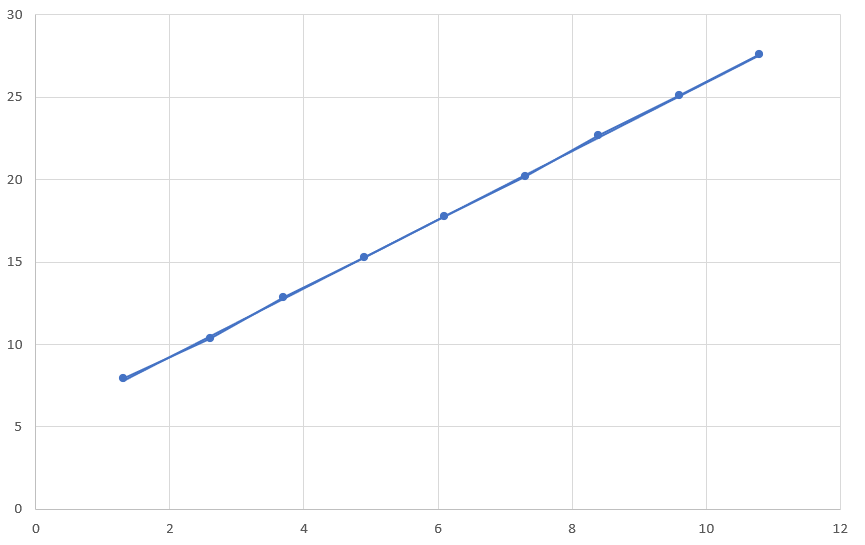
\includegraphics[width=1\linewidth]{graph.png}\\
   
\end{center}


\center{\textbf{Обсуждение результатов и выводы}}
\begin{flushleft}
    {
В ходе работы мы определили модуль Юнга для проволоки:
    

\begin{itemize}
	\item \underline{$ E = \left( 18,3 \cdot {10}^{10} \pm 0,7 \cdot {10}^{10} \right) \text{ Па}, \left( \varepsilon = 4 \% \right)   $}
\end{itemize}
Полученный модуль Юнга в пределах погрешности совпадает с табличным значением модуля Юнга железа. Можно сделать вывод, что исследуемым материалом было железо. На точность результата достаточно сильно влияет погрешность измерений параметров установки (длина проволоки, ее диаметр и т.д).
    }
\end{flushleft}


















\end{document}